\documentclass[12pt]{article}
\usepackage[a4paper]{geometry}
%\userpackage[top=1 in, bottom=1.25 in, left=1.1 in, rigth=1.1 in] {geometry}
%\usepackage[paperwidth=17cm, paperheight=22.5cm, bottom=2.5cm, right=2.5cm]{geometry}
\usepackage[utf8]{inputenc}
%\usepackage[a4paper, top=2.5cm, bottom=2.5cm, left=2.2cm, right=2.2cm]
%{geometry}
%\usepackage[myheadings]{fullpage}
\usepackage{fancyhdr}
\usepackage{lastpage}
%\usepackage{float}
\usepackage{graphicx, wrapfig, subcaption, setspace, booktabs}
\usepackage{graphicx}
\usepackage[T1]{fontenc}
\usepackage[font=small, labelfont=bf]{caption}
%\usepackage{fourier}
\usepackage[protrusion=true, expansion=true]{microtype}
\usepackage[english]{babel}
\usepackage{sectsty}
\usepackage{url, lipsum}
\usepackage[T1]{fontenc}
\usepackage{icomma}
\usepackage{siunitx}
\usepackage{ragged2e}
\usepackage{amsmath}
\usepackage{comment}
\usepackage{enumerate}
%\usepackage{changepage}
\usepackage{anysize}




\newcommand{\HRule}[1]{\rule{\linewidth}{#1}}
\onehalfspacing
\setcounter{tocdepth}{5}
\setcounter{secnumdepth}{5}

%-------------------------------------------------------------------------------
% HEADER & FOOTER
%-------------------------------------------------------------------------------


\begin{comment}
-Udledninger
$$
\begin{aligned}


\end{aligned}
$$

-Opgavetekst
\begin{figure}[H]
\includegraphics[width=0.5\textwidth]{"path"}
\end{figure} 


-Opgave billede med tekst
\begin{figure}[H]
\caption{"Billedtekst"}
\includegraphics[width=0.5\textwidth]{"path"}
\end{figure} 

-Værdier
$\\

$


\end{comment}
\begin{document}

\begin{titlepage}

\title{ \normalsize 
		%\begin{figure}
        \begin{center}
        
\includegraphics[height=6cm]{Logo.jpg}
        \end{center}
       % \end{figure}
        \LARGE \textsc{\textbf{Universidad De Sonora}} \\ \bigskip
		\Large División de Ciencias Exactas y Naturales \\
        Licenciatura En Física \\ \bigskip
        \bigskip
        Física Computacional I
		\\ [0.1cm]  
		\HRule{2pt} \\
		\Large \textbf{{Reporte de Actividad 3}} \\
        \textit{\textbf{"Medición de Propiedades de la Atmósfera con el Apoyo de Sondeos por Globos Meteorológicos"}}
		\HRule{2pt} \\
		\normalsize \vspace*{0.001\baselineskip}}
        
\date{\bigskip \Large Hermosillo, Sonora  \hspace*{\fill}  Febrero 14 de 2018}

        
\author{
		\Large\textbf{ César Omar Ramírez Álvarez} \\ \bigskip
        \\ \bigskip
       \Large Profr. Carlos Lizárraga Celaya}
       \end{titlepage}
       \maketitle
       

\newpage
\pagestyle{plain}

\section*{Introducción}
La práctica de la semana ha consistido en trabajar apoyándonos con los datos de sondeos atmosféricos que organiza la Universidad de Wyoming. Dichos datos se han tomado del sitio web de la Universidad con la finalidad de analizar el comportamiento que se ha tenido en \textit{"Camborne Observations"} en Europa los días 22 de Junio y 22 de Diciembre de 2017.\\

Como es el caso de las prácticas anteriores, esta práctica también está encaminada a seguir practicando con el entorno de programación que ofrece Jupyter Notebook para programar con Phyton, también se han agregado las bibliotecas auxiliares que son Pandas, Numpy y Pyplot de Matplotlib que nos ofrecen distintas herramientas para organizar la información obtenida y realizar graficas como sea necesario y requerido.\\

Durante el desarrollo del presente reporte se mostrarán los elementos necesarios para la realización de la práctica, así como los fundamentos teóricos, procedimientos, conclusiones y bibliografías.

\section*{Fundamentos}

Primeramente, vamos a conocer sobre lo que es un sondeo atmosférico y algunas de sus características. Un sondeo atmosférico es una medición de la distribución vertical de las propiedades físicas de la columna atmosférica, como presión, temperatura, velocidad del viento y dirección del viento, contenido de agua líquida, concentración de ozono, contaminación y otras propiedades. Tales mediciones se realizan en una variedad de formas que incluyen detección remota y observaciones en el sitio.\\

La herramienta mas utilizada para realizar los sondeos es el globo meteorológico, este aparato durante el día se encarga de recabar información de las propiedades físicas antes mencionadas, tomando datos por radiosondeos a diferentes alturas. Entre muchas otras funciones que cumplen los sondeos es validar los modelos para el pronóstico del tiempo.\\

Al mencionar que el globo toma datos a diferentes alturas de la atmósfera, debemos recordar la teoría de la primera práctica, podemos rescatar de ella el hecho de que la atmósfera se encuentra clasificada en capas según la relación que cumplen sus propiedades (temperatura, presión, densidad, etc.) y a diversas alturas nos encontramos con estas 5 principales capas: 1.- Tropósfera (0 a 12 km), 2.- Estratósfera (12 a 50 km), 3.- Mesósfera (50 a 80 km), 4.- Termósfera (80 a 700 km) y 5.- Exósfera (700 a 10,000 km). Sabiendo esto es mas que suficiente para comprender y complementar la información generada con los datos de la práctica.


\section*{Análisis de Datos}


Como dijimos en un principio, trabajamos apoyándonos con los datos de sondeos atmosféricos que organiza la Universidad de Wyoming. Dichos datos se han tomado del sitio web de la Universidad con la finalidad de analizar el comportamiento que se ha tenido en \textit{"Camborne Observations"} en Europa los días 22 de Junio y 22 de Diciembre de 2017. Descargamos los dos archivos que contiene a los datos y observamos la estructura que tienen, verificando no tener datos basura y datos que nos puedan causar problemas al momento de leer desde Jupyter Notebook. Debemos de cargar las bibliotecas de Pandas, Numpy y Matplotlib antes de iniciar con cualquier lectura de datos desde nuestro archivo en Jupyter Notebook. A continuación, mostramos la estructura de los datos:
\begin{center}
	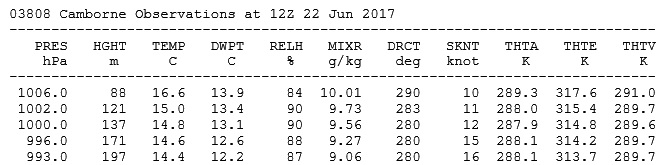
\includegraphics[height=3.5cm]{DatosJ.jpg}
    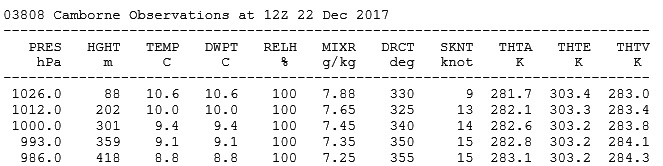
\includegraphics[height=3.5cm]{DatosD.jpg}
\end{center}
Como nos podemos percatar, las primeras filas no aportan nada (excepto la que nombra cada una de las columnas), por lo que, para evitar problemas al momento de leer, nos saltaremos las primeras 5 filas y nombraremos una por una cada columna.\\

Primeramente añadiremos las bibliotecas:
\begin{center}
	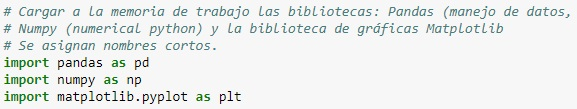
\includegraphics[height=2.5cm]{Bibliotecas.jpg}
\end{center}
Posteriormente procedemos a leer y hacer los saltos necesarios:
\begin{center}
	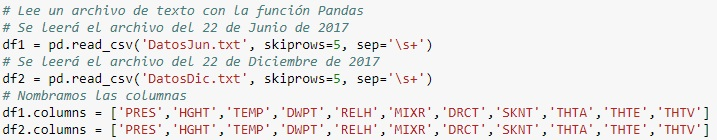
\includegraphics[height=2.5cm]{Lectura.jpg}
\end{center}
Verificamos que al leer ya nos aparezcan los nombres de las columnas y los datos:
\begin{center}
	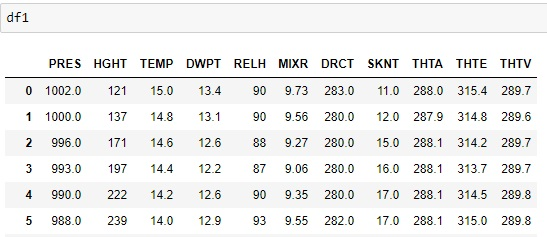
\includegraphics[height=3.5cm]{DatJ.jpg}
    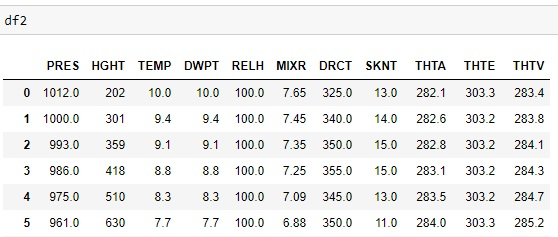
\includegraphics[height=3.5cm]{DatD.jpg}
\end{center}
En la estructura de los datos nos dimos cuenta que al final de documento tenemos datos incompletos, por lo que evitaremos que se lean para evitar posibles errores usando lo siguiente para cada mes:
\begin{center}
	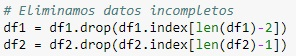
\includegraphics[height=1cm]{Eliminados.jpg}
\end{center}
Comprobamos que nuestros datos son valores numéricos para poder operar:
\begin{center}
	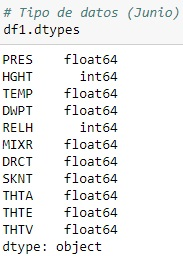
\includegraphics[height=3.5cm]{tipoj.jpg} <--Junio y Diciembre-->       
    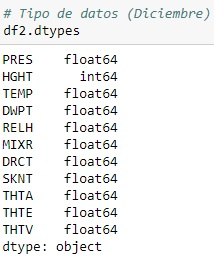
\includegraphics[height=3.5cm]{tipod.jpg}
\end{center}
Al tener todos nuestros datos como valores numéricos no tenemos problema para iniciar con las gráficas requeridas.

\section*{Resultados}
 Para la presentación de las gráficas se mostrarán tanto el código como la gráfica para ambos meses. Considerando que para una de ellas se tuvo que trabajar con limites en sus ejes para poder apreciar y comprender mejor la apreciación de lo que muestran.\\
 
La primera de ellas será una gráfica de la variación de la presión con respecto a la altura:
\begin{center}
	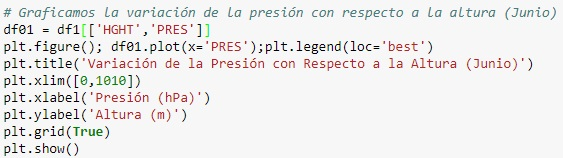
\includegraphics[height=2cm]{dj1.jpg} \hspace*{\fill}
    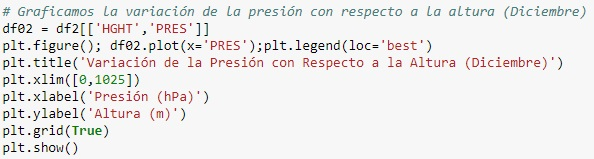
\includegraphics[height=2cm]{dd1.jpg}
\end{center}
\begin{center}
	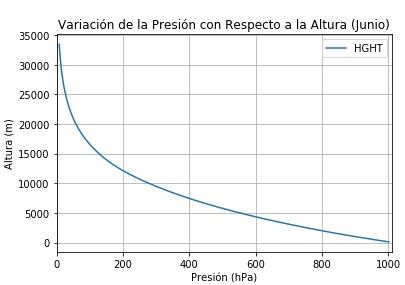
\includegraphics[height=5cm]{gj1.jpg}  \hspace*{\fill}
    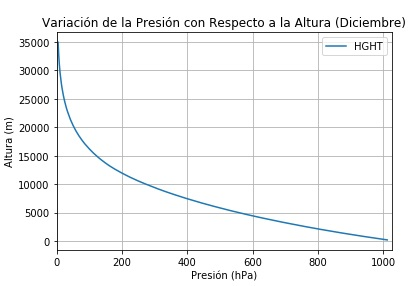
\includegraphics[height=5cm]{gd1.jpg}
\end{center}
Se hace notorio el descenso de presión mientras mas alejados de la superficie de la Tierra nos encontremos.\\

Continuando, tenemos una gráfica de la variación de la temperatura con respecto a la altura:
\begin{center}
	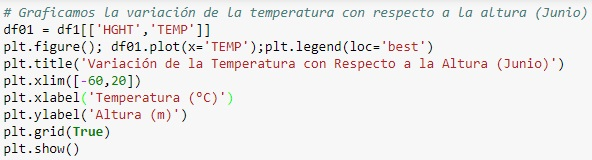
\includegraphics[height=2cm]{dj2.jpg} \hspace*{\fill}
    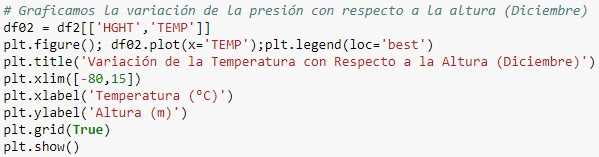
\includegraphics[height=2cm]{dd2.jpg}
\end{center}
\begin{center}
	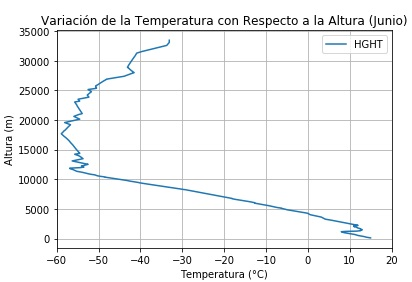
\includegraphics[height=5cm]{gj2.jpg}  \hspace*{\fill}
    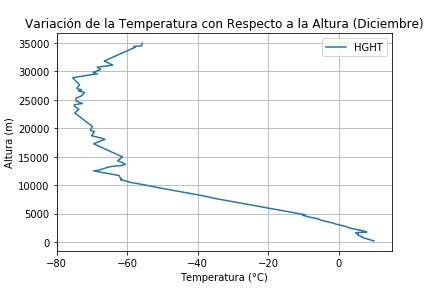
\includegraphics[height=5cm]{gd2.jpg}
\end{center}
La pregunta propuesta  \textit{¿Hay cambios significativos en la tropopausa entre las dos fechas?} Podemos afirmar que si se presenta un cambio. Según conocemos la tropopausa se encuentra entre los 9 y 17 km, observamos las graficas y alrededor de esos valores encontramos un descenso (pareciera que es el máximo) y aumento de nuevo conforme ganamos mas altura. \\

Siguiendo, podemos ver la gráfica de la temperatura y temperatura de rocío, como función de la altura:
\begin{center}
	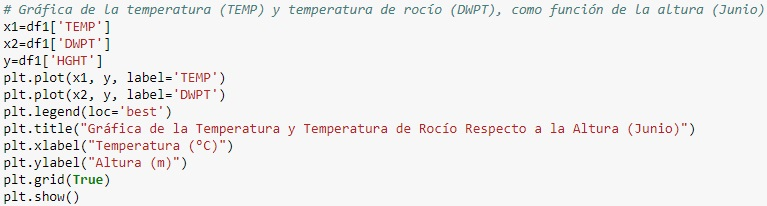
\includegraphics[height=2cm]{dj3.jpg} \hspace*{\fill}
    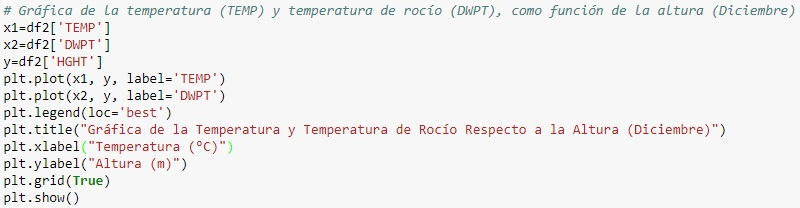
\includegraphics[height=2cm]{dd3.jpg}
\end{center}
\begin{center}
	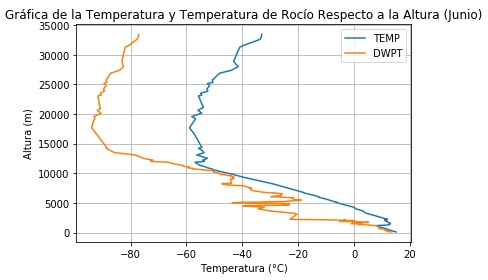
\includegraphics[height=4cm]{gj3.jpg}  \hspace*{\fill}
    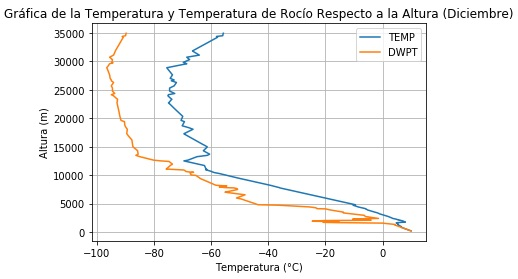
\includegraphics[height=4cm]{gd3.jpg}
\end{center}
Según las graficas podemos inferir que desde cierta capa (Estratósfera) estas dos temperaturas llevan el mismo comportamiento, salvo que la temperatura de rocío permanece mas baja respecto a la temperatura.\\

La próxima grafica nos presenta la rapidez de los vientos en nudos usando todos los datos proporcionados:
\begin{center}
	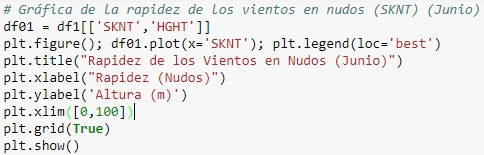
\includegraphics[height=2cm]{dj4.jpg} \hspace*{\fill}
    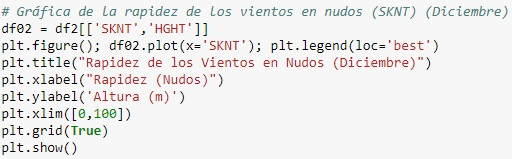
\includegraphics[height=2cm]{dd4.jpg}
\end{center}
\begin{center}
	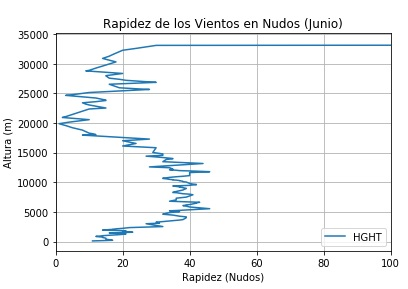
\includegraphics[height=5cm]{gj4.jpg}  \hspace*{\fill}
    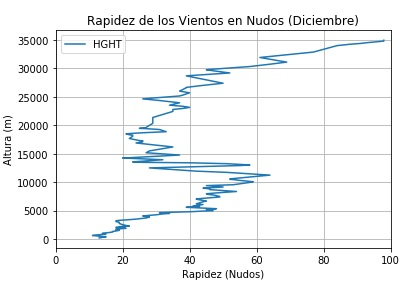
\includegraphics[height=5cm]{gd4.jpg}
\end{center}
Con respecto a la rapidez de los vientos, observamos que no tenemos un "buen comportamiento" es decir, constante, aunque en Junio es mejor comportado que en Diciembre.\\
\\

Y por último, tenemos la gráfica de la humedad relativa como función de la altura:
\begin{center}
	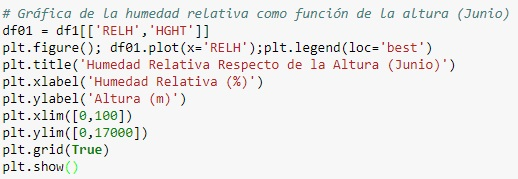
\includegraphics[height=2cm]{dj5.jpg} \hspace*{\fill}
    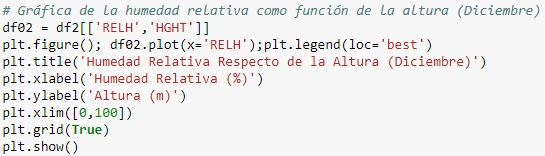
\includegraphics[height=2cm]{dd5.jpg}
\end{center}
\begin{center}
	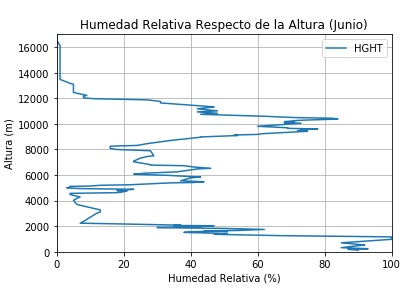
\includegraphics[height=5cm]{gj5.jpg}  \hspace*{\fill}
    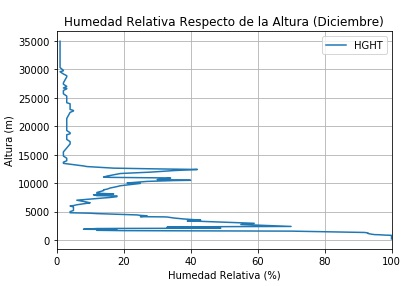
\includegraphics[height=5cm]{gd5.jpg}
\end{center}
En ambas graficas es notoria su variacion, aunque se estabiliza a menor altura en Diciembre.
\section*{Conclusión}
Desde el moento que leí la práctica pense que todo iba a ser fácil, pero con el desarrollo me di cuenta que no era del todo fácil, pues al mostrarnos una cantidad grande de datos el analizarlos y clasificarlos para leerlos se puede complicar demasiado, segun los límites de cada quién, por lo qué se ocupó visitar frecuentemente varios sitios de complementación para poder tener listos los datos al moento de realizar sus graficas respectivas.\\

La parte gráfica no se me complico, pues ya se habia estado trabajando con ellas en actividades anteriores y partí de esos códigos para realizar éstas.\\

En cuanto a la teoría de la actividad me pareció muy interesante y muy útil para presentarse de éstam manera, la de analizar datos de este tipo y ver lo que realmente sucede a diversas alturas de la atmósfera y a su vez, complementando las prácticas anteriores.\\

Puedo decir que se cumplió el obejtivo, pues se llegó a realizar la práctica con éxito y sobre todo, darnos cuenta que el análisis de datos puede complicarse según los límites y herramientas de cada quién.


\section*{Bibliografía}
\begin{itemize}
\item  Atmospheric sounding. (2018). En.wikipedia.org. Recuperado el 13 de Febrero de  2018, desde https://en.wikipedia.org/wiki/Atmospheric\_sounding
\item  Atmosphere of Earth. (2018). En.wikipedia.org. Recuperado el 13 de Febrero de  2018, desde https://en.wikipedia.org/wiki/Atmosphere\_of\_Earth
\item  Tutorial de pandas | Pybonacci. (2018). Pybonacci.org.  Recuperado el 8 de Febrero de  2018, desde http://www.pybonacci.org/tag/tutorial-de-pandas/
\item  Usando El Tipo DataFrame de Python Pandas. (2018). Relguzman.blogspot.mx. Recuperado el 8 de Febrero de  2018, desde http://relguzman.blogspot.mx/2015/06/usando-el-tipo-dataframe-de-python.html
\end{itemize}

\section*{Apéndice}
\begin{enumerate}
\item ¿Cuál es tu opinión general de esta actividad?\\
\textit{Me parecio muy interesante por que complementamos la actividad anterior, pero esta vez se trabajo más con análisis y preparación de datos para despues graficar.}
\item ¿Qué fue lo que más te agradó? ¿Lo que menos te agradó?\\
\textit{En general me gustó todo, pero el hecho de graficar de una gran cantidad de datos me parece sorprendente, la verdad cada práctica parece gustarme más Phyton como enguaje de programación, algo que en un principio me desagradó fue cuando tuvimos que preparar los datos (evitar cosas innecesarias), pues puede perderse mucho tiempo.}
\item ¿Que consideras que aprendiste en esta actividad? \\
\textit{En general, formas de darle formato a las gráficas (color, estilo, etiquetas, etc) y comandos para análisis y acomodo de datos.}
\item ¿Qué le faltó? ¿O le sobró? \\
\textit{Estuvo muy completa para el nivel en el que vamos, considero que conforme avanzemos seguiremos aprendiendo y complementando mas sobre la programación en Phyton.}
\item ¿Que mejoras sugieres a la actividad?\\
\textit{Siempre mostrar bibliografía de donde apoyarnos, no solo para la parte teórica si no para comando y herramientas posibles a utilizar}.
\end{enumerate}

\end{document}
